\chapter{Read Me}

You can remove this file (and this chapter) after you finish working on the documentation. Consider it as a cheat sheet for your (probably first) documentation and also as a guideline for using \LaTeX{} and Overleaf. I am sure you will use \LaTeX{} even for other occasions (like writing a CV more professionally, writing your diploma project, writing an article, for a poster, and so on). Besides this file, the others can be kept because I expect you to follow the guidelines and the structure I have created for you. You just have to fill in the information under some sections and answer to a couple of questions.

\noindent
{\color{red} \rule{\linewidth}{0.5mm} }
The most important thing I am expecting from you while writing this documentation is to learn and make an idea of how such a tool works. You will not receive a lower mark if the documentation doesn't look the best, but I expect you to \textbf{use Overleaf}. 

\noindent
{\color{red} \rule{\linewidth}{0.5mm} }

Remember: 
\begin{itemize}
    \item In order to save your changes, you have to recompile the project from the 'Recompile' green button.
    
    \item A disadvantage of using Overleaf (free edition) in big teams is that the owner of the project can share the project with only one editor, so the other teammates won't be able to make changes to the files. But you can split your documentation into tasks and you can combine your work in the end.
    
    \item Each one of you will have to upload the documentation on Campus. I will read only one documentation from each team (they have to be the same) and I will read only the answers to the \textbf{conclusions} chapter (I expect them to be unique because I assume each one of you has a different opinion).
    
    \item Your documentation should not be longer than 12 pages. I know for some of you it's harder to come up with a lot of words, but remember that the documentation also has \textbf{tables}, \textbf{code sequences}, \textbf{figures}.
    
\end{itemize}

\section{How to insert code?}

Did you know you can list code in \LaTeX{}? You just have to copy-paste it from the IDE inside a \textbf{lstlisting} element. You can provide a caption which explains that sequence of code. The caption doesn't have to be long, but please make it explanatory enough. Please do not copy the entire code, but we'll discuss about this later.

I've attached a short snip of code from one of my previous projects. You can see that the caption is pretty clear and it is longer than just a couple of words, which is good for the reader, who has to understand not only what the code does, but \textbf{\textit{why}} you have included a specific code sequence. 

\begin{lstlisting}[caption={Checking if the user has selected the role in the application checking a radioButton according to his role (doctor or patient). If any radioButton has been selected, the register button changes is colour and becomes enabled.}, language=Java]
    
    radioGroup = findViewById(R.id.rol);
    registerButton = findViewById(R.id.registerButton);
    radioGroup.setOnCheckedChangeListener((group, checkedId) -> {
        RadioButton checkedRadioButton = radioGroup.findViewById(checkedId);
        boolean isChecked = checkedRadioButton.isChecked();
        if(!isChecked){
            setRegisterButtonStyle(false, "#ffe082");
        } else {
            setRegisterButtonStyle(true, "#ffb300");
        }
    });
\end{lstlisting}

Also, we can choose to add a list of all code sequences, a list of all tables, and also a list with all figures, but this kind of lists are recommended for more elaborate documents. I remember the fact that \textbf{you shouldn't write a document with more than 12 pages}. 

\section{How to insert equations?}

You can also list equations (probably the score's formula, right?).

\begin{equation}
z = (x - u)/s
\end{equation}

\section{How to insert tables?}

\begin{table}[ht]
\centering
\begin{tabular}{|l|l|l|l|l|l|l|l|}
\hline
\textbf{Nr} & \textbf{CPU}  & \textbf{Cores} & \textbf{Clock} & \textbf{RAM} & \textbf{OS} & \textbf{...} & \textbf{Score} \\ \hline
1           & Core i5 7600K & 4/4            & 3.50           & 4096         & Win10 Home  & ...          & 1205           \\ \hline
2           & Ryzen 7 1700X & 8/16           & 3.00           & 8192         & Win8.1 Pro  & ...          & 1622           \\ \hline
\end{tabular}
\caption{Your caption describing the table.}
\label{example-table}
\end{table}

You definitely don't have to worry about learning or understanding details about how tables work in Overleaf, the syntax used to generate a table, and other things. Just use a generator (I suggest you to use \cite{table-generator}) and your job will be a lot easier. The table \ref{example-table} is pretty good.

\section{How to insert images?}

You can set a lot of parameters for the pictures you choose to insert in the documentation. You can find out more about them here \cite{image-documentation}. For figure \ref{statistics-diagram} I chose the width and also I wanted to keep the aspect ratio unchanged. Inside the folder called \textbf{figures} you can store the figures you want to use. Don't delete the ones that are there now because they are used on the first page.

\begin{figure}[H]
    \centering
    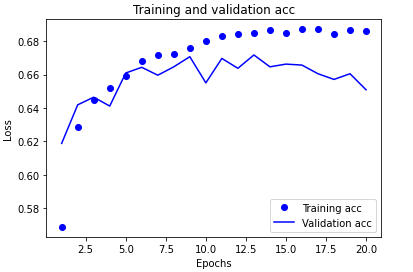
\includegraphics[width=11cm,keepaspectratio]{figures/training.png}
    \caption{Monitoring the training and validation accuracy. In this figure we can see that the model starts overfitting at around the 10th epoch.}
    \label{statistics-diagram}
\end{figure}